\documentclass[oneside,final]{hcmut-report}
\usepackage{array,tabularx,listings,pgfplots,etoolbox}
\pgfplotsset{compat=1.18}
\lstset{basicstyle=\ttfamily\small,breaklines=true,frame=single,
  columns=fullflexible,keepspaces=true,showstringspaces=false}
\emergencystretch=2em
\setcounter{tocdepth}{2}
\coursename{Introduction to Artificial Intelligence}
\reporttype{Homework 2 Report}
\title{Chesss}
\reporttime{October 2026}
\stuname{%
  & Nguyễn Quốc Hiệu & 2352344 \\
  & Quách Hoàng Phú & 2352922 \\
  & Chu Nguyễn Tuấn Anh & 2352022 \\
  & Lê Hoàng Chí Vĩ & 2353336 \\
  & Vũ Hải Tuấn & 2353280 \\
  & Nguyễn Lê Đăng Vinh & 2353330 \\
  & Dương Nguyễn Tấn Đạt & 2352222 \\
  & Đỗ Thái Phong & 2352903 \\
}
% No instructor name was supplied; keep the original class and omit that row.
\makeatletter
\patchcmd{\coverpage}{Advisor(s): \@advisor \\}{}{}{\PackageError{report}{Cannot omit the advisor row}{Check the template cover macro.}}
\makeatother

\begin{document}
\coverpage
\pagenumbering{roman}
\section*{Member List and Workload}
\addcontentsline{toc}{section}{Member List and Workload}
\begin{table}[ht]
\centering\small
\caption*{Group members and completion of the agreed workload.}
\label{tab:members}
\begin{tabularx}{\textwidth}{>{\raggedright\arraybackslash}p{1.7cm}>{\raggedright\arraybackslash}p{3.4cm}p{1.9cm}>{\raggedright\arraybackslash}X}\toprule
\textbf{Student ID} & \textbf{Full name} & \textbf{Workload} & \textbf{Main work}\\\midrule
2352344 & Nguyễn Quốc Hiệu & 100\% & Problem formulation, application architecture, and request validation. \\
2352922 & Quách Hoàng Phú & 100\% & Negamax, Alpha-beta pruning, move ordering, and iterative deepening. \\
2352022 & Chu Nguyễn Tuấn Anh & 100\% & Position evaluation, quiescence search, and exchange diagnostics. \\
2353336 & Lê Hoàng Chí Vĩ & 100\% & MCTS tree structure, adversarial UCT selection, and value backup. \\
2353280 & Vũ Hải Tuấn & 100\% & Guided rollouts, immediate-mate screening, and controlled ablations. \\
2353330 & Nguyễn Lê Đăng Vinh & 100\% & English interface, human/AI game modes, and comparison display. \\
2352222 & Dương Nguyễn Tấn Đạt & 100\% & Automated tests, certified fixtures, timed runs, and game records. \\
2352903 & Đỗ Thái Phong & 100\% & Result analysis, report preparation, reproducibility, and packaging. \\
\bottomrule\end{tabularx}
\end{table}

The table gives the main task allocation. All eight members have equal agreed
workload and share integration, peer checking, and documentation. Each 100\%
entry means completion of that member's agreed tasks.

\clearpage

\section*{Abstract}
\addcontentsline{toc}{section}{Abstract}
We built a browser-based chess application for Homework 2 to study how two
search methods choose moves: Alpha-beta pruning and Monte Carlo Tree Search
(MCTS). The application supports human--AI games, AI--AI games, and manual
position exploration. It also lets users compare both algorithms on the same
position without changing the board. We implemented the searches ourselves
and used python-chess for legal moves and game outcomes.

Our study combines short tactical tests with complete, color-swapped games.
The earlier extended experiments contain 360 position searches and 20 games. Alpha-beta solved all 12 enhanced tactical
cases at one and five seconds and won all four games in the five-second
subset. MCTS was less reliable on the bounded tactical objectives, and its
guided version did not consistently outperform the original random-rollout
version. One recorded example shows why these results need care: MCTS chose
to capture a rook rather than follow a faster forced mate. The move failed the
fast-mate test, but that alone does not make it a losing move. A follow-up adds immediate-mate screening, 912 controlled ablation
searches, and matched-start games with unfinished results kept separate.
The project
provides a working simulation and a reproducible comparison of these two
implementations; the small, selected test set does not establish a general
ranking of chess engines.
\clearpage

\tableofcontents
\listoffigures
\clearpage
\pagenumbering{arabic}

\section{Introduction}
Chess is a useful setting for studying search because the board is visible,
the rules are fixed, and each decision leads to several possible replies.
The difficult part is deciding which continuations deserve attention when
there is not enough time to examine the whole game tree. This project studies
two ways to spend that limited time. Alpha-beta searches a depth-limited tree
and skips branches that cannot affect its decision. MCTS builds evidence by
repeatedly sampling possible continuations.

Our goal was to make both algorithms playable and their decisions inspectable.
The interface shows the suggested moves, Alpha-beta's best line and completed
depth, and MCTS's visits and sampled values. We also recorded experiments so
that the comparison could be checked from data rather than judged from one
interesting game.

The main questions are practical: Can each algorithm return a legal move
within the allocated time? How do their decisions change with a larger budget?
Do the enhanced heuristics help on the chosen tests? What can tactical tests
and full-game results tell us, and where do those measurements stop being useful?

\subsection{Problem formulation}
A state includes the pieces, the player to move, castling rights, the en-passant
square, move counters, and known history. The legal moves are the available
actions. Applying one of them produces the next state. A tersminal result is a
win, loss, or draw; a nonterminal state needs an estimate because the search
usually stops before the game ends. The objective is to choose a useful legal
move within a specified thinking budget.

We retain history because two identical-looking boards can have different
rights or draw conditions. Loading a FEN restores a position and its counters,
but not the earlier repetitions. For consistency, the simulator automatically
claims an available threefold-repetition or fifty-move draw. This policy is
shared by both algorithms and the experiment runner.

\section{Background and Algorithms}
In this report, a \emph{ply} is one player's move, and search depth counts
plies. The \emph{root} is the position from which the AI is choosing its next
move. A \emph{rollout} is a simulated continuation used to estimate a position.
These terms describe search, not different rules of chess.

\subsection{Minimax and Negamax}
Minimax chooses a move under the assumption that the opponent will choose
its best reply. In a zero-sum game, a score that is good for one player is bad
for the other. Negamax uses that relationship to express both turns with one
recurrence:
\[
 V(s,d)=\max_{a\in A(s)}\left[-V(T(s,a),d-1)\right].
\]
Here $A(s)$ is the set of legal moves and $T(s,a)$ applies a move. Terminal
positions receive a result-based score. At a nonterminal depth cutoff, the
program uses its static evaluation from the player-to-move perspective.
Negamax is a convenient form of minimax; Alpha-beta supplies the pruning.

\subsection{Alpha-beta pruning}
Alpha-beta maintains bounds on the scores that still matter to the current
decision. After a promising move raises $\alpha$, another branch can be stopped
once its bound shows that it cannot improve the choice. In our code, the
cutoff is the explicit condition $\alpha\geq\beta$. For a fixed tree and
leaf evaluation, pruning preserves the minimax result while avoiding some
work. Knuth and Moore give a formal analysis of this method~\cite{knuthmoore}.

A full depth-$d$ tree can require $O(b^d)$ work, where $b$ is the branching
factor. Favorable move ordering can reduce Alpha-beta's work substantially,
with the ideal case approaching $O(b^{d/2})$; the worst case is still
exponential. This is why we try promising moves first.

Our search starts at depth one and increases the depth while time remains.
The previous iteration's best move is tried first, followed by ordered captures,
promotions, and other legal moves. If time runs out during a deeper iteration,
the engine keeps the result from the last completed iteration. If none
completes, it returns a legal fallback and does not invent a score.
Checkmate is scored as $-100000+\text{ply}$ for the losing player; the small
ply adjustment makes the search prefer a shorter forced win. Draws score zero.
\begin{lstlisting}[caption={The main Alpha-beta search in Negamax form.}]
search(state, depth, alpha, beta, ply):
    stop if the deadline or cancellation flag is reached
    if terminal: return the mate or draw score
    if depth == 0: return quiescence or static evaluation
    best = -infinity
    for move in ordered legal moves:
        push(move)
        value = -search(child, depth-1, -beta, -alpha, ply+1)
        pop(move), including when search is interrupted
        update best move and its principal variation
        alpha = max(alpha, value)
        if alpha >= beta: count a cutoff and stop this loop
    return best score and principal variation
\end{lstlisting}

\subsubsection{Quiescence in the enhanced version}
A fixed depth can stop in the middle of an exchange and make a capture look
better than it is. The enhanced version uses quiescence at the depth cutoff:
it continues captures and promotions, and searches every legal evasion when
the king is in check. This extension uses the same bounds and terminal checks.
It is capped at six extra plies; at the cap it returns a static score even if
the position is still in check, so the horizon is reduced rather than removed.

One test makes this difference easy to see. At depth one, the baseline takes
a defended pawn with its queen and overlooks the rook's reply. The enhanced
search avoids that capture. This verifies a specific tactical improvement;
it does not prove that the enhanced version is always stronger. The engine
exports normal nodes, quiescence nodes, evaluations, and cutoffs separately.

\subsection{Monte Carlo Tree Search}
MCTS estimates the value of moves from repeated sampled continuations.
Our implementation uses UCT to balance revisiting promising moves with trying
less-explored alternatives. This tree-based use of bandit selection follows
the approach introduced by Kocsis and Szepesv\'ari~\cite{uct}. One iteration
has four stages:
\begin{enumerate}
\item \textbf{Selection:} follow UCT choices through the existing tree.
\item \textbf{Expansion:} add one untried legal action. Each action is added only once at a node.
\item \textbf{Simulation:} play a bounded continuation and obtain a terminal result or cutoff estimate.
\item \textbf{Backup:} add that value and one visit to every node on the selected path.
\end{enumerate}

Each node stores its player to move, untried actions, child nodes, visits $N$,
and summed utility $W$. Utilities are always measured for the root player.
To account for the opponent, selection changes the sign of the exploitation
term while keeping exploration positive:
\[
 \operatorname{UCT}(j)=\sigma\frac{W_j}{N_j}
 +\sqrt{2}\sqrt{\frac{\ln(\max(1,N_{parent}))}{N_j}},\qquad
 \sigma=\begin{cases}+1&\text{root player's turn},\\-1&\text{opponent's turn}.\end{cases}
\]
This means the opponent seeks a lower root utility but still explores.
Unvisited children receive priority. The implementation uses only completed
simulations for backup, so a rollout interrupted by the deadline contributes
no result. At the end, the AI chooses the root child with the most visits,
then breaks ties by mean utility and stable move order.
\begin{lstlisting}[caption={One MCTS search under a time budget.}]
repeat until time runs out:
    copy the root position with its known history
    select UCT children through fully expanded nodes
    expand one untried legal action
    simulate a bounded continuation
    reward = +1 for a root win, -1 for a loss, 0 for a draw
    at a nonterminal cap: reward = tanh(E_root / 400)
    add the completed reward and a visit along the path
choose the most-visited root action
\end{lstlisting}

The baseline uses random expansion and at most 40 random rollout plies.
The enhanced version scores expansion moves with a simple tactical policy
and uses 12-ply guided rollouts. It rewards captures, promotions, castling,
central pawn/minor-piece moves, checks, and immediate mates, while penalizing
currently attacked destinations. Rollouts still choose a random move 15\%
of the time. The danger estimate is made on the pre-move board, so it can
miss a discovered attack or a pin.

The current enhanced version also checks immediate mates at the root before
sampling. It returns a proven mate in one directly, or removes moves that
allow an immediate opposing mate when a safe alternative exists. This is
an exact, bounded preprocessing step, not a replacement for UCT. Its cost
is included in the thinking budget; an interrupted scan does not apply a
partial filter. The original enhanced runs below predate this guard.

The nonterminal reward $\tanh(E_{root}/400)$ is a bounded heuristic value,
not a calibrated win probability. A large value can reflect favorable
material without proving a forced win. MCTS therefore depends on both its
sampling policy and its cutoff evaluation. With $I$ iterations, rollout
length $L$, and selection depth $D$, its main work grows roughly as
$O(I(L+D))$, with additional costs for legal moves and board copies. More
samples provide more evidence under that policy, but a short, biased rollout
can still miss an important reply.

\section{Implementation}
\subsection{Architecture and chess rules}
The program separates the interface, request handling, and search so that
each part has a clear job. The browser sends a position and settings to the
local server; the server checks them and calls the selected search.
\begin{center}
\fbox{\texttt{index.html}} $\longrightarrow$
\fbox{\texttt{app.py}} $\longrightarrow$
\fbox{\texttt{engine.py}}
\end{center}
\begin{table}[ht]
\centering\small
\caption{Responsibilities of the main project files.}
\begin{tabularx}{\textwidth}{p{.31\textwidth}X}\toprule
\textbf{File} & \textbf{Responsibility}\\\midrule
\texttt{engine.py} & Evaluation, iterative Alpha-beta, quiescence, and UCT MCTS.\\
\texttt{app.py} & Local HTTP server, input checks, legal state reconstruction, and search cancellation.\\
\texttt{index.html} & Board, game modes, controls, history, comparison cards, and exports.\\
\texttt{experiments.py} & Serial searches, tactical answer certification, and paired games.\\
\texttt{analyze\_results.py} & Tables, seed statistics, paired-start resampling, and plot data from recorded results.\\
\texttt{test\_homework.py} & Search, rules, reference-answer, statistics, and HTTP checks.\\\bottomrule
\end{tabularx}
\end{table}

We use python-chess 1.999, with chess 1.11.2, for legal moves, push/pop,
game outcomes, FEN, and PGN~\cite{pythonchess}. Both searches are our own
implementations. Relying on one rules library keeps the comparison focused
on search rather than differences between two sets of chess rules. Castling,
en passant, all four promotions, checkmate, stalemate, and draw conditions
are handled through that library.

The server accepts legal moves only and listens on loopback. One search runs
at a time. A cancellation flag stops pending work, and a generation counter
prevents an old reply from being applied after a new game or reset. Search
copies retain the known move history; moves pushed during Alpha-beta are
always undone, including on interruption. The application uses Python's
standard library and plain HTML/CSS/JavaScript, with no frontend build step.

\subsection{Shared evaluation and configuration choices}
Both algorithms use the same evaluator for the selected version. The base
score is White-relative, using material values of 100 for a pawn, 320 for a
knight, 330 for a bishop, 500 for a rook, and 900 for a queen. One hundred
centipawns equals one pawn in this scoring scale. Negamax changes the sign
for the side to move, and MCTS changes it for the root player.

The baseline adds simple positional bonuses. With files and oriented ranks
numbered 0--7, and Black's ranks mirrored, let
\[
 C=7-\tfrac12|2f-7|-\tfrac12|2r-7|.
\]
Pawn bonus is $8r+3C$, knight/bishop bonus is $10C$, and king bonus is
$10C$ in an endgame or $-8C$ otherwise. We treat total nonpawn material at
most 2600 as the endgame threshold. Other pieces receive no base positional
bonus, and the final score is rounded to integer centipawns.

The enhanced version adds a bishop-pair bonus of 30; penalties of 12 for
doubled and isolated pawns; a passed-pawn bonus of $15+4r^2$; and attack
mobility weighted 4 for knights/bishops, 2 for rooks, and 1 for queens.
Rooks receive 10 on a semi-open file or 18 on an open file. Outside the
endgame, king protection adds 12 per nearby forward pawn and 30 for a
back-rank king on files b/c/g/h, then subtracts 8 per attacked neighboring
square. The mobility term counts attacked squares excluding friendly pieces,
not fully legal moves. These are small, readable heuristics rather than a
trained model or an external engine.

Keeping baseline and enhanced settings lets us measure the combined effect
of these choices. Since several features change together, their comparison
cannot identify which individual feature caused a difference.

\subsection{Interface and supported game modes}
The interface uses English and presents match controls before optional AI
analysis. Users can play against either algorithm, watch two AIs, or explore
a position manually. In human mode, the opponent responds automatically,
including White's opening if the user chooses Black. In AI mode, users can
run a match, advance one move, or pause. Advanced settings choose each side's
algorithm, the shared version, the thinking budget, and the MCTS seed.

The analysis view searches the same unchanged position with both algorithms
in sequence. Arrows identify their suggestions. Alpha-beta reports its
completed depth, principal variation, and pruning counters; MCTS reports
completed simulations and root-action visits and utility. The two scores
have different units and are kept separate. Move history, undo, board flip,
FEN loading, PGN export, and comparison JSON support further inspection.
\begin{figure}[ht]
\centering
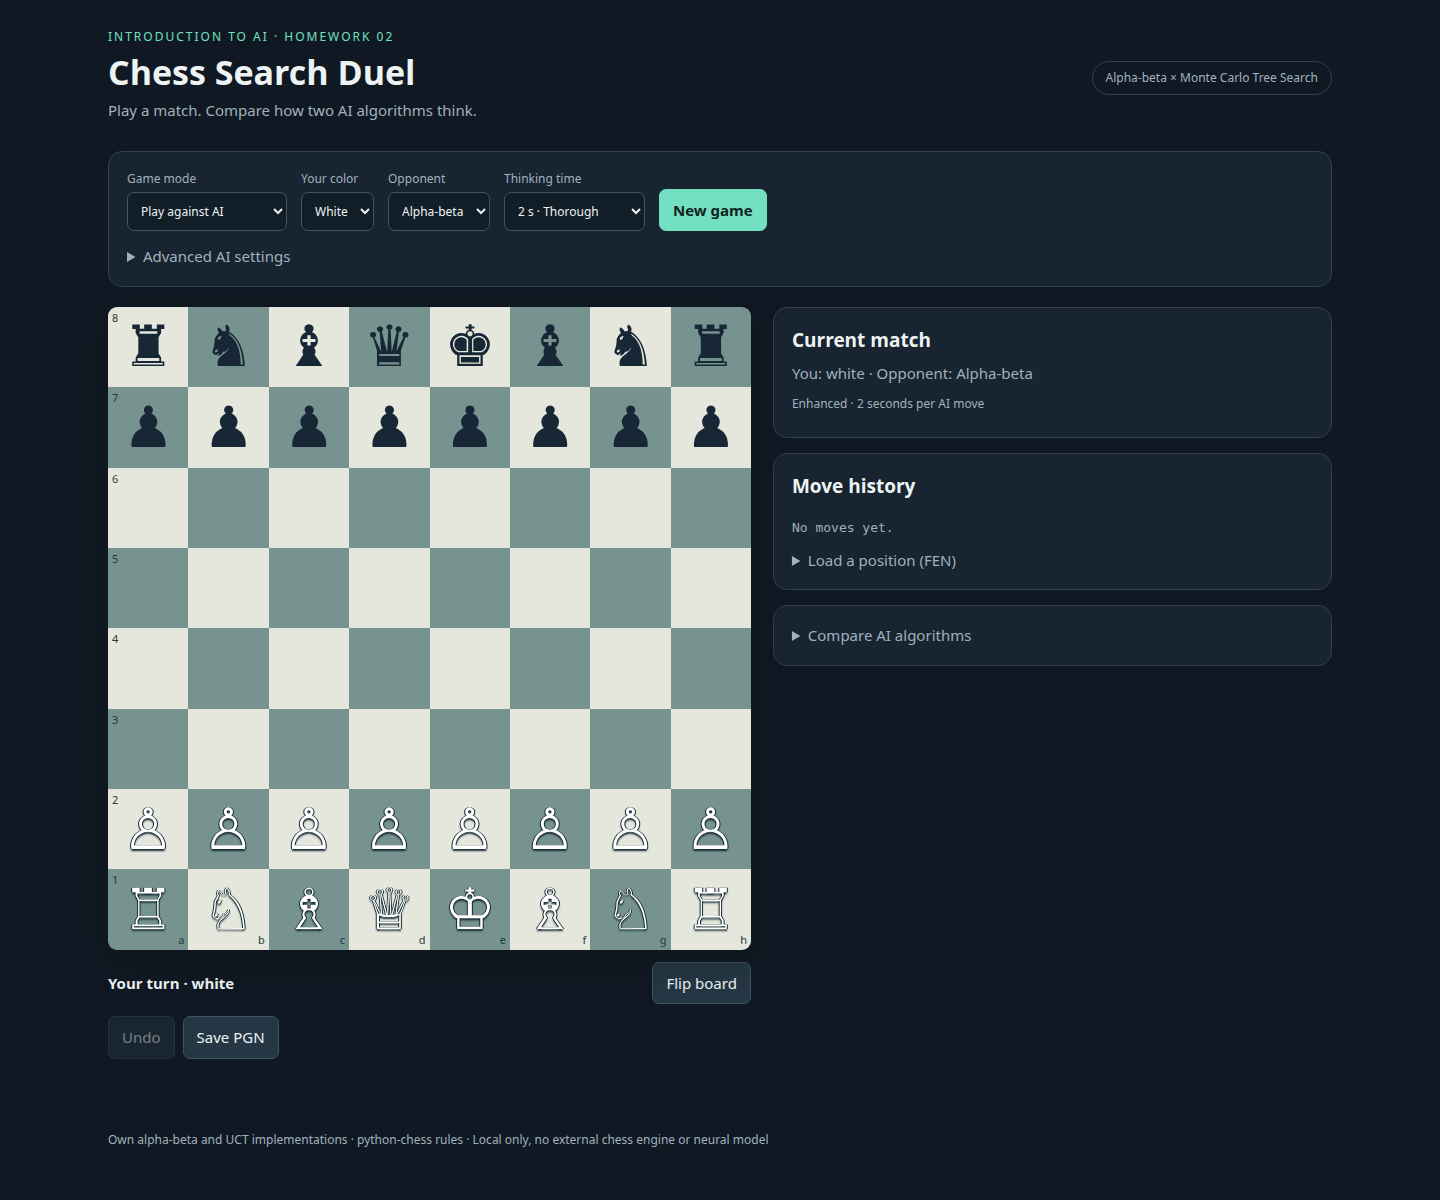
\includegraphics[width=.91\textwidth]{gui.png}
\caption{The implemented English interface. Match controls and history are visible, while AI comparison is available in a separate panel.}
\label{fig:gui}
\end{figure}

\section{Experimental Method}
The four extended runs below use the earlier, frozen implementation. Its
exact \texttt{engine.py} and \texttt{experiments.py} are preserved under
\texttt{extended\_results/source/}. The follow-up study is reported
separately and uses the current implementation. Old measurements are not
relabelled as results of the upgraded engine.

\subsection{Datasets and thinking budgets}
The main extended study contains 360 position searches. We test enhanced
settings at 0.1, 1, and 5 seconds, and baseline settings at 0.1 and 1 second.
At each budget, Alpha-beta runs once per case and MCTS runs with seeds 7--11.
We also run 16 enhanced games at 0.5 seconds from eight starts and four
at 5 seconds from two starts, with the algorithms' colors swapped at every
start. A ply cap of 60 is fixed before these games begin.

The tactical set has three constructed king/queen/rook placements. Each is
tested for attack, defense, and their color mirrors, giving 12 cases. They
are more demanding than the earlier mate-in-one checks: the attacker must
force mate in two, and two of the three attacking placements have a unique
first move. These cases are useful diagnostics, but the mirrors do not
turn three placement families into twelve independent samples.

The eight game starts include four opening-derived positions and four
endgames. The five-second subset uses the Italian and Queen's Gambit starts.
These are convenience samples, and the budget subsets are different. Their
aggregate scores therefore do not isolate the effect of increasing time.
Earlier demonstration runs are retained separately and summarized in
Appendix~\ref{app:earlier}.

\subsection{Checking answers without judging moves by eye}
The tactical answers come from a separate bounded AND/OR solver that uses
no static evaluation and does not call either timed search. At an attacking
node, one winning continuation is enough; at a defending node, every legal
reply must still lead to mate. The solver checks every root action and
exports all accepted actions in \texttt{reference\_answers.json}.

For attack, success means forcing mate within three plies. For defense,
success means preventing the opponent from forcing mate within the next
three plies after the chosen move. The defensive test does not establish
an eventual draw or the globally best move. This distinction matters when
the reader does not know chess well: the program can verify the stated
short-horizon objective, but it cannot turn that result into a verdict on
the whole game. All legal moves in the recorded PGNs were also replayed
and checked.

\subsection{Fairness, timing, and reproducibility}
Searches run serially and receive the same allocated budget and rules.
The evaluator version is also shared. Time measurement includes copying
the board, checking outcomes, evaluating positions, and sampling continuations;
it excludes rendering and reference-answer certification. A proven mate
can finish early. Small overruns are recorded rather than silently scored
as time forfeits. Seeds fix random choices, but time-limited runs can still
complete different numbers of iterations on another machine.

The measurements were collected on WSL2 with an Intel Core i7-12700H,
Python 3.14.4, and chess 1.11.2. The engine was frozen throughout the study.
Each run records its configuration, start/end UTC, versions, and hashes
of the engine, runner, and input fixtures. An interrupted startup pilot
that overlapped test execution is excluded from the analysis. The four
completed runs and their full CSV, JSONL, and PGN files are included.

Game score is $(\text{wins}+0.5\,\text{draws})/\text{games}$. We distinguish
natural draws from games stopped at the ply cap. For the eight-start study,
we resample whole color-swapped pairs to describe variation among the
selected starts. Individual moves are not treated as independent games.
The two-start five-second subset is too small for a useful precision claim.

\section{Results}
\label{sec:results}
\begin{center}\small
\begin{tabular}{llrrrr}\toprule
Variant & Engine & Budget & Mate / trials & Defense / trials & Overall\%\\\midrule
Enhanced & Alpha-beta & 0.1s & 4/6 & 4/6 & 66.7 \\
Enhanced & MCTS & 0.1s & 11/30 & 13/30 & 40.0 \\
Enhanced & Alpha-beta & 1s & 6/6 & 6/6 & 100.0 \\
Enhanced & MCTS & 1s & 0/30 & 3/30 & 5.0 \\
Enhanced & Alpha-beta & 5s & 6/6 & 6/6 & 100.0 \\
Enhanced & MCTS & 5s & 1/30 & 4/30 & 8.3 \\
Baseline & Alpha-beta & 0.1s & 0/6 & 3/6 & 25.0 \\
Baseline & MCTS & 0.1s & 2/30 & 14/30 & 26.7 \\
Baseline & Alpha-beta & 1s & 6/6 & 5/6 & 91.7 \\
Baseline & MCTS & 1s & 2/30 & 10/30 & 20.0 \\
\bottomrule\end{tabular}\end{center}
\subsubsection*{Search cost and MCTS stability}
\begin{center}\small\begin{tabular}{llrrrr}\toprule
Variant & Budget & AB depth & AB tactical nodes & MCTS simulations & Distinct moves\\\midrule
Enhanced & 0.1s & 2 & 315 & 33 & 3.92 \\
Enhanced & 1s & 3 & 2196.5 & 403.5 & 2.92 \\
Enhanced & 5s & 3.5 & 7205 & 1896 & 2.83 \\
Baseline & 0.1s & 2 & 0 & 14 & 4.58 \\
Baseline & 1s & 3 & 0 & 136.5 & 4.42 \\
\bottomrule\end{tabular}\end{center}
Depth, tactical nodes and simulations are medians. Distinct moves is the mean number
of different suggestions across five seeds per position; it ranges from 1 to 5.
These work counters measure different operations and must not be compared as equivalent nodes.
\subsubsection*{Wall-clock measurements}
\begin{center}\small\setlength{\tabcolsep}{4pt}\begin{tabular}{lrrrrr}\toprule
Variant & Budget & AB median (s) & MCTS median (s) & MCTS p95 (s) & Max overrun (ms)\\\midrule
Enhanced & 0.1s & 0.1001 & 0.1001 & 0.1003 & 0.762 \\
Enhanced & 1s & 0.6521 & 1.0000 & 1.0003 & 0.416 \\
Enhanced & 5s & 2.6608 & 5.0000 & 5.0001 & 0.274 \\
Baseline & 0.1s & 0.1001 & 0.1001 & 0.1004 & 0.526 \\
Baseline & 1s & 0.6397 & 1.0001 & 1.0004 & 0.702 \\
\bottomrule\end{tabular}\end{center}
Small overrun is measured and retained, not scored as a time-forfeit loss. Early proven mates can leave allocated time unused.
\subsubsection*{Color-swapped games}
\begin{center}\small\begin{tabular}{rrrrrrr}\toprule
Budget & Starts & Games & AB wins & Draws & AB losses & AB score\%\\\midrule
0.5s & 8 & 16 & 10 & 6 & 0 & 81.2 \\
5s & 2 & 4 & 4 & 0 & 0 & 100.0 \\
\bottomrule\end{tabular}\end{center}
For 0.5s, resampling the 8 paired starts 5,000 times gives a descriptive 95\% percentile interval [65.6\%, 93.8\%] for Alpha-beta's score.
This resampling keeps both colors together and uses seed 2352344. It reflects
variation among the selected starts, not a representative chess population.
No interval is reported for the two-start 5s subset: it is too small to support a useful precision claim.
\begin{figure}[ht]\centering
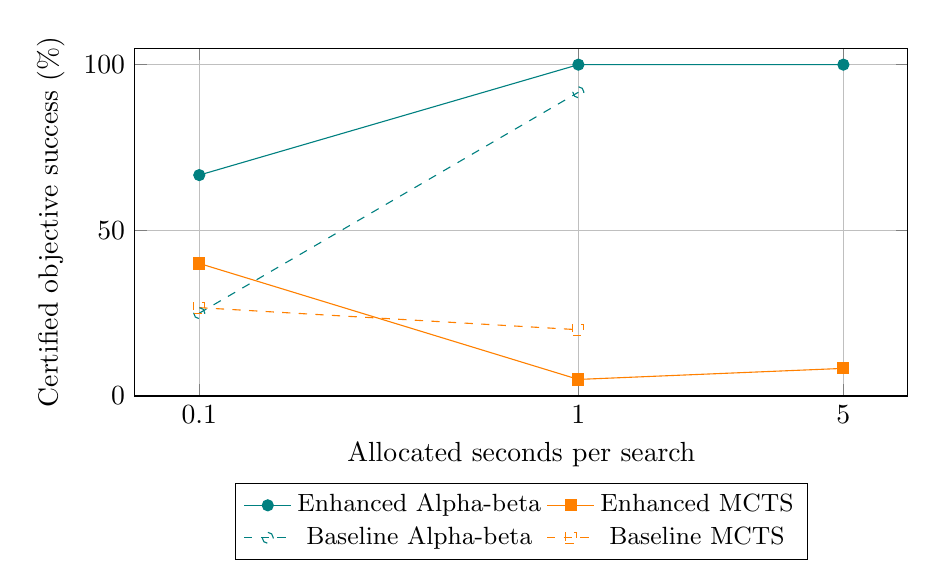
\begin{tikzpicture}\begin{axis}[width=.94\textwidth,height=6cm,xmode=log,
xlabel={Allocated seconds per search},ylabel={Certified objective success (\%)},
xtick={.1,1,5},xticklabels={0.1,1,5},ymin=0,ymax=105,grid=major,
legend style={at={(.5,-.25)},anchor=north,legend columns=2,font=\small}]
\addplot[teal,mark=*] coordinates {(0.1,66.667) (1.0,100.000) (5.0,100.000)};
\addlegendentry{Enhanced Alpha-beta}
\addplot[orange,mark=square*] coordinates {(0.1,40.000) (1.0,5.000) (5.0,8.333)};
\addlegendentry{Enhanced MCTS}
\addplot[teal,dashed,mark=o] coordinates {(0.1,25.000) (1.0,91.667)};
\addlegendentry{Baseline Alpha-beta}
\addplot[orange,dashed,mark=square] coordinates {(0.1,26.667) (1.0,20.000)};
\addlegendentry{Baseline MCTS}
\end{axis}\end{tikzpicture}
\caption{Success on the fixed certified corpus, combining attack and defense objectives. Baseline was tested at 0.1 and 1 seconds only. Lines connect measured budgets and do not predict intermediate performance.}\end{figure}


\section{Discussion}
The certified test answers a limited, objective question about each selected move.
It does not use agreement between the two engines as a correctness label.
A high agreement rate can reflect the same mistake; different suggestions can both satisfy the objective.
At 5s, enhanced Alpha-beta succeeds on 6/6 attacking trials and 6/6 defensive trials. Alpha-beta runs once on each of six cases per objective.
At 5s, enhanced MCTS succeeds on 1/30 attacking trials and 4/30 defensive trials. The MCTS denominators include five seeds on each of six cases.
\paragraph{Configuration and cost tradeoff.}
At 1s, Alpha-beta's combined certified success is 91.7\% for baseline and 100.0\% for enhanced.
At 1s, MCTS's combined certified success is 20.0\% for baseline and 5.0\% for enhanced.
Median completed MCTS simulations at 1s are 136.5 baseline versus 403.5 enhanced. These differ because both rollout length and per-action policy cost changed.
Quiescence extends tactical lines but consumes work that could otherwise increase nominal depth.
Guided simulations introduce useful tactical bias and additional move-scoring cost.
A configuration's effect is therefore a measured cost/quality tradeoff, not a guarantee that more features improve every position.
\paragraph{Seed variation and agreement.}
At 5s, MCTS chooses 2.83 distinct moves on average across five seeds per case; its average modal share is 60.0\%, and agreement with Alpha-beta is 5.0\%.
Low variation is repeatability, not proof of correctness. With multiple certified answers, disagreement is not automatically an error.
Completed-visit counts and sampled utility should be inspected together; root utility is not a calibrated win probability.
Alpha-beta centipawns and MCTS utility remain different units and are not ranked on a common score scale.
\paragraph{Concrete, auditable examples.}
Examples use seed 7, the first scheduled seed; aggregate tables include all five seeds and both colors.
\begin{quote}\small\textbf{Corner net / force\_mate / original}. Accepted UCI moves: \texttt{a4a1}, \texttt{a4c6}, \texttt{a4e4}.
Alpha-beta selects \texttt{a4a1}, satisfies the certified objective, and reports completed depth 3 in 0.186s.
MCTS (seed 7) selects \texttt{a4a1}, satisfies the certified objective, and reports 2316 completed simulations in 5.000s.
\end{quote}
\begin{quote}\small\textbf{Corner net / avoid\_mate / original}. Accepted UCI moves: \texttt{h1h2}, \texttt{h8f8}, \texttt{h8h2}.
Alpha-beta selects \texttt{h8f8}, satisfies the certified objective, and reports completed depth 4 in 5.000s.
MCTS (seed 7) selects \texttt{h8f8}, satisfies the certified objective, and reports 2449 completed simulations in 5.000s.
\end{quote}
\begin{quote}\small\textbf{Unique queen maneuver / force\_mate / original}. Accepted UCI moves: \texttt{e3e7}.
Alpha-beta selects \texttt{e3e7}, satisfies the certified objective, and reports completed depth 3 in 0.284s.
MCTS (seed 7) selects \texttt{e3g1}, fails the certified objective, and reports 1913 completed simulations in 5.000s.
\end{quote}
\begin{quote}\small\textbf{Unique queen maneuver / avoid\_mate / original}. Accepted UCI moves: \texttt{d8c8}, \texttt{g1c1}, \texttt{g1d1}, \texttt{g1e1}, \texttt{g1g6}, \texttt{g1g7}.
Alpha-beta selects \texttt{g1d1}, satisfies the certified objective, and reports completed depth 4 in 5.000s.
MCTS (seed 7) selects \texttt{g1g7}, satisfies the certified objective, and reports 1457 completed simulations in 5.000s.
\end{quote}
\begin{quote}\small\textbf{Narrow rook defense / force\_mate / original}. Accepted UCI moves: \texttt{c4c1}.
Alpha-beta selects \texttt{c4c1}, satisfies the certified objective, and reports completed depth 3 in 0.234s.
MCTS (seed 7) selects \texttt{c4a2}, fails the certified objective, and reports 1892 completed simulations in 5.000s.
\end{quote}
\begin{quote}\small\textbf{Narrow rook defense / avoid\_mate / original}. Accepted UCI moves: \texttt{d7d1}, \texttt{d7g7}.
Alpha-beta selects \texttt{d7g7}, satisfies the certified objective, and reports completed depth 4 in 5.000s.
MCTS (seed 7) selects \texttt{d7d8}, fails the certified objective, and reports 1972 completed simulations in 5.000s.
\end{quote}
\paragraph{Why the fast-mate metric is not a strength verdict.}
In the unique queen maneuver, the certified line is \texttt{e3e7 d8c8 e7c7}: Qe7+, Kc8, Qc7 mate. There is only one legal defensive reply after Qe7+.
MCTS instead captures the rook with \texttt{e3g1} (Qxg1), giving it 234 visits and mean utility 0.892; the certified first move gets 25 visits and utility 0.336.
The capture improves material but does not force mate within the benchmark's three-ply bound. This measurement alone does not establish that the capture loses or is globally inferior.
Alpha-beta's mate score favors a shorter forced win. MCTS gives every terminal win the same utility and its cutoff rewards material; it has no explicit mate-speed reward.
Those scoring choices and sampled continuations can favor a slower material gain. The observed visit/utility allocation is evidence of the choice; attributing all failures to this mechanism would require further controlled tests.
Increasing computation can reinforce a policy's preferred objective instead of improving a different diagnostic score. Full-game outcomes must therefore accompany the tactical table.
\paragraph{Game results and practical meaning.}
A color-swapped game tests the full decision sequence, while a certified tactic tests one bounded decision. Neither substitutes for the other.
The 0.5s and 5s studies use different sets of starts. Their aggregate game scores therefore cannot isolate the causal effect of increasing time.
At 0.5s, 3 of 16 games reached the cap and 3 were natural draws. Alpha-beta's score is 81.2\%; the median game length is 37.5 plies.
At 5s, 0 of 4 games reached the cap and 0 were natural draws. Alpha-beta's score is 100.0\%; the median game length is 28.5 plies.
Report wins, natural draws and capped draws separately before treating a score as playing strength.
The selected endgames and opening positions are convenience starts, not a random chess population.
The first move of a fixture may belong to Black; swapping engine colors preserves that same starting state.
\paragraph{What remains unproven.}
The three constructed placement families are low-material diagnostic tasks. Mirror cases and repeated seeds are correlated, and five seeds do not resolve rare failures.
No reference engine evaluates arbitrary middlegame moves, no external puzzle corpus is held out, and no Elo estimate is justified.
Longer simulations and more visits do not guarantee an optimal chess move. The contribution is transparent, independently checked bounded tactics and reproducible comparison of these implementations.


\section{Follow-up Improvements Within the Homework Scope}
The follow-up keeps the two search algorithms visible and changes only
features that can be explained, tested, and measured in this assignment.
We add an exact immediate-mate guard to enhanced MCTS, expose independent
search settings for experiments, broaden the diagnostic tasks, and stop
counting unfinished benchmark games as draws. We do not add a neural
network, opening book, endgame database, Elo calibration, multiplayer
service, or a large external-engine evaluation pipeline.

\subsection{An exact guard around MCTS}
Before UCT sampling, the enhanced engine checks every root action for an
immediate mate. A proven mate is returned directly and is labelled as a
proof in the interface; it is not presented as a sampled utility. Otherwise,
the guard checks each opponent reply for immediate mate. When at least one
alternative avoids this immediate loss, proven losing actions are excluded
from the root. If every action loses immediately, the engine retains legal
choices. The guard uses the same deadline and cancellation checks as MCTS,
and an interrupted scan does not apply an incomplete filter.

This is MCTS with bounded tactical preprocessing. It does not solve deeper
combinations, replace the four MCTS stages, or turn the rollout policy into
an optimal opponent. The original baseline remains available for comparison.

\subsection{Broader diagnostics and controlled ablations}
We now use 24 positions: the earlier 12 bounded tactical cases, four
mate-in-one cases, and eight material cases. The material cases cover a
queen exchange trap, a rook exchange trap, an undefended queen capture,
and pawn promotion, each with a color mirror. Their answers are computed
by exhaustively enumerating the root action and the opponent's reply.
The accepted actions maximize the worst-case material gain over that
short continuation. Terminal wins and losses take priority, and draws
receive zero. This diagnostic does not use our positional evaluator and
does not declare a globally best chess move.

An initial pilot used a capture case that ended in an insufficient-material
draw. Its label also accepted quiet moves, making the capture diagnostic
uninformative. We added a pawn, certified the unique capture independently,
and repeated the complete run. The pilot is retained locally and excluded
from the reported analysis and submission data.

The serial ablation run contains 912 searches at 0.1 and 0.5 seconds.
Alpha-beta runs once per case and configuration; MCTS uses seeds 7, 8, and 9.
The four Alpha-beta configurations independently enable enhanced evaluation
and quiescence. The five MCTS configurations isolate the cutoff evaluator,
random versus guided policy, 12 versus 40 rollout plies, and the new guard.
For example, comparing ``MC guided 12'' with ``MC guided 40'' changes only
the rollout cap, while comparing ``MC guided 12'' with ``MC guided 12 guard''
changes only the root guard. Timing includes that guard's work.

In the table, AB means Alpha-beta and MC means MCTS. The numbers 12 and 40
are rollout caps in plies.
\begin{center}\small\setlength{\tabcolsep}{4pt}
\begin{tabular}{lrrrrr}\toprule
Configuration & Seconds & Mate & Defense & Material & Combined\%\\\midrule
AB basic & 0.1 & 4/10 & 4/6 & 8/8 & 66.7 \\
AB evaluation only & 0.1 & 4/10 & 2/6 & 8/8 & 58.3 \\
AB quiescence only & 0.1 & 8/10 & 4/6 & 8/8 & 83.3 \\
AB both & 0.1 & 8/10 & 4/6 & 8/8 & 83.3 \\
MC random basic 12 & 0.1 & 12/30 & 6/18 & 18/24 & 50.0 \\
MC random enhanced 12 & 0.1 & 12/30 & 3/18 & 18/24 & 45.8 \\
MC guided 12 & 0.1 & 10/30 & 8/18 & 19/24 & 51.4 \\
MC guided 40 & 0.1 & 10/30 & 13/18 & 16/24 & 54.2 \\
MC guided 12 guard & 0.1 & 15/30 & 10/18 & 19/24 & 61.1 \\
AB basic & 0.5 & 10/10 & 5/6 & 8/8 & 95.8 \\
AB evaluation only & 0.5 & 10/10 & 4/6 & 8/8 & 91.7 \\
AB quiescence only & 0.5 & 10/10 & 6/6 & 6/8 & 91.7 \\
AB both & 0.5 & 10/10 & 5/6 & 6/8 & 87.5 \\
MC random basic 12 & 0.5 & 14/30 & 3/18 & 21/24 & 52.8 \\
MC random enhanced 12 & 0.5 & 12/30 & 7/18 & 16/24 & 48.6 \\
MC guided 12 & 0.5 & 12/30 & 3/18 & 17/24 & 44.4 \\
MC guided 40 & 0.5 & 17/30 & 10/18 & 22/24 & 68.1 \\
MC guided 12 guard & 0.5 & 12/30 & 5/18 & 18/24 & 48.6 \\
\bottomrule\end{tabular}\end{center}
Combined percentages describe this fixed diagnostic mix. They are not playing-strength ratings.


The controls reveal tradeoffs that the earlier baseline/enhanced comparison
could not separate. At 0.1 seconds, adding quiescence with the basic
evaluator raises Alpha-beta's attacking success from 4/10 to 8/10, but its
defensive success remains 4/6. At 0.5 seconds, quiescence with
the basic evaluator succeeds on all six defenses, versus five for the
basic search. Adding the richer evaluator is not consistently beneficial
on these selected cases. These results support a targeted extension, not
an unconditional claim that every enhancement makes the engine stronger.

The immediate-mate subset gives the clearest guard result. At 0.1 seconds,
guided 12-ply MCTS succeeds on 8/12 seeded trials, versus 12/12 with the
guard. In those guarded mate-in-one trials, the move is established by
exact checking and requires no simulations. At 0.5 seconds both versions
already achieve 12/12. Over all 24 cases, the guard changes success from
51.4\% to 61.1\% at 0.1 seconds and from 44.4\% to 48.6\% at 0.5 seconds.
The modest overall change is consistent with the guard's narrow purpose:
it addresses immediate tactics, not the mate-in-two objectives.

Longer guided rollouts illustrate the time tradeoff. At 0.1 seconds,
40-ply MCTS has a median 15.5 simulations and 54.2\% combined success,
compared with 37 simulations and 51.4\% for 12 plies. However, the longer
rollout succeeds on only 5/12 immediate-mate trials, versus 8/12 for the
shorter one. At 0.5 seconds, 40 plies reaches 68.1\%, compared with 44.4\%
for 12 plies, despite median simulation counts of 77 versus 192.5.
The result depends on the objective as well as cost. We retain the short
interactive default and report the alternative instead of tuning it to
this small constructed corpus.

The material objective also exposes a measurement limitation. On the
original promotion case, enhanced Alpha-beta at 0.5 seconds chooses
\texttt{h1g2}; its completed five-ply line is
\texttt{h1g2 h8g7 a7a8q g7f6 g2f3}. It plans to promote later, but receives
zero immediate material gain under the two-ply diagnostic, while immediate
queen promotion gains 800. This is a failure of the stated short-term
objective, not proof that the king move loses the game. Adding more kinds
of tasks broadens coverage; it does not remove the need to state what each
metric actually measures.

\subsection{Matched game starts and honest unfinished results}
The current engines play 16 additional color-swapped games from four starts:
Italian opening, Queen's gambit, rook ending, and knight versus pawns.
Both budgets, 0.1 and 0.5 seconds per move, use those same four states and
paired seed schedule. The cap increases from 60 to 120 plies. A capped
nonterminal game now has PGN result \texttt{*}, is counted as unfinished,
and is excluded from the completed-game score. The table also shows the
range of possible scores if every unfinished game later becomes a loss
or a win for Alpha-beta. That prevents a cap from silently inflating draws.

\begin{center}\small\setlength{\tabcolsep}{4pt}
\begin{tabular}{rrrrrrr}\toprule
Seconds & Games & AB wins & Draws & AB losses & Unfinished & Score range\%\\\midrule
0.1 & 8 & 5 & 3 & 0 & 0 & 81.2--81.2 \\
0.5 & 8 & 6 & 2 & 0 & 0 & 87.5--87.5 \\
\bottomrule\end{tabular}\end{center}
The range assigns every unfinished game first a loss and then a win for Alpha-beta. It is a censoring bound, not a confidence interval.


All 16 new games ended naturally. At 0.1 seconds, Alpha-beta wins five
and draws three, for a score of 81.25\%. At 0.5 seconds it wins six and
draws two, for 87.5\%. There are no capped games in this measured run,
so both endpoints of the censoring range coincide. The improved cap policy
is still covered by an automated test that deliberately stops a nonterminal game.

The same starts remove one confound from the earlier comparison of
budgets, but four selected starts remain a small sample. Timing is still
machine-dependent, and a completed-game percentage can be selective when
many games remain unfinished. We therefore report unfinished counts and
score bounds alongside the outcomes rather than estimating Elo.

\subsection{What is improved and what remains}
The new guard prevents a limited class of sampling mistakes, while the
ablation controls separate the cost and benefit of individual settings.
Exchange and promotion diagnostics broaden the original tactical coverage;
matched starts make the budget comparison clearer; unfinished results
improve the interpretation of game scores. The tests additionally verify
independent quiescence/evaluation settings, exact mate selection, rejected
immediate losses, exhaustive material labels, and censored-game arithmetic.

Finite search depth, a six-ply quiescence cap, short simulated continuations,
and handcrafted evaluation remain deliberate limits. A substantially
stronger chess engine or a general strength ranking would require a much
larger development and evaluation effort. Those extensions are outside
this homework's goal of implementing and comparing two understandable
search methods.

\section{Verification and Limitations}
The project has 27 standard-library tests. They check Alpha-beta's mate
choices for both colors and baseline agreement with an unpruned minimax
search on small trees. They also check the enhanced poisoned-pawn defense,
evaluation symmetry, MCTS's unique actions and adversarial selection,
fixed-iteration seed repeatability, independent evaluation/quiescence settings,
immediate-mate screening, cancellation, legal fallback, and
preservation of the original board and history.

Integration checks cover illegal inputs, repeated-position draws, castling,
en passant, every promotion, PGN, capped games, local HTTP requests, and
cross-origin rejection. Further tests check the certified tactical answers
and paired-start resampling. Chrome checks exercised actual moves,
comparison without board changes, reset during a search, promotion, undo,
and AI-match pause. The 52 recorded benchmark games were replayed legally,
including the 20 earlier extended games and the 16 follow-up games.

These checks support correct behavior on the tested cases. They do not
prove optimal decisions in arbitrary positions. Quiescence still has a
finite horizon, MCTS can miss replies, and both depend on modest heuristics.
The tactical corpus is constructed and small; repeated seeds and mirrored
cases are correlated. We have not evaluated arbitrary moves against a
reference engine or estimated Elo. The added material diagnostic is still
only a two-ply objective, and the additional fixtures remain constructed. The application is a local simulator,
and timing results remain sensitive to host load.

\section{Conclusion}
The submitted program meets the requested chess topic with a GUI, explicit
Alpha-beta pruning and MCTS implementations, and recorded comparisons.
On our selected tests, enhanced Alpha-beta was more reliable at finding
short forced tactics and performed better in the paired games. The MCTS
results show a useful lesson: a guided rollout and more simulations can
make a choice more stable without making it better under a different
tactical objective. We therefore report both the observed choices and
the limits of the measurements.

A larger follow-up could use an independently sourced puzzle corpus and
more paired starts. The current ablations already separate evaluator,
rollout policy, and rollout length, while matched starts improve the short-budget
comparison. Broader independent data would be needed to generalize those findings. Those would extend the evidence;
they are not results claimed by this submission.

\section*{References and Acknowledgements}
\addcontentsline{toc}{section}{References and Acknowledgements}
The supplied \texttt{Chess}, \texttt{chessmc}, and \texttt{Chess-engine}
repositories informed our design study. Their useful ideas included
separating rules from search, exposing visits and values, and making board
controls easy to inspect. We implemented the searches and interface
independently, without copying their source, images, or model weights.
Their original remote URLs were not established from the supplied copies.

This report uses the supplied HCMUT report template from the hcmut-report project. The
class and university logo are included with the template's licence and
source information. The template's sample content is replaced by our project
report. Details are recorded in \texttt{THIRD\_PARTY\_NOTICES.md}.
\begin{thebibliography}{9}
\bibitem{knuthmoore} D. E. Knuth and R. W. Moore.
\emph{An Analysis of Alpha-Beta Pruning}. Artificial Intelligence, 6(4),
293--326, 1975. \url{https://doi.org/10.1016/0004-3702(75)90019-3}.
\bibitem{uct} L. Kocsis and C. Szepesv\'ari.
\emph{Bandit Based Monte-Carlo Planning}. ECML, 282--293, 2006.
\url{https://sites.ualberta.ca/~szepesva/papers/ecml06.pdf}.
\bibitem{pythonchess} N. Fiekas and contributors.
\emph{python-chess documentation}, chess 1.11.2.
\url{https://python-chess.readthedocs.io/en/latest/}.
\bibitem{template} hoang-himself.
\emph{HCMUT Report Template}. Source revision supplied with the assignment
workspace: \texttt{350906b86be7adae1c953217029cbe12ad4f6ac5}.
\url{https://github.com/hoang-himself/hcmut-report}.
\end{thebibliography}

\appendix
\section{Earlier Demonstration Runs}
\label{app:earlier}
The earlier runs used 12 positions, including four simple mate-in-one cases,
with budgets of 0.1 and 0.25 seconds and five MCTS seeds. Each configuration
also played eight color-swapped games from two opening starts. These records
remain separate from the extended study and retain their original source
hashes. They show how the initial comparison motivated the harder tests;
they do not enlarge the independent sample of the main study.
\subsection{Historical baseline}
\begin{center}
\begin{tabular}{rrrrrr}
\toprule
Budget & Engine & Mate solve & Median (s) & p95 (s) & Game score\\
\midrule
0.10 & Alpha-beta & 100\% & 0.10004 & 0.10014 & 87.5\% \\
0.10 & MCTS & 100\% & 0.10007 & 0.10018 & 12.5\% \\
0.25 & Alpha-beta & 100\% & 0.25002 & 0.25009 & 100.0\% \\
0.25 & MCTS & 100\% & 0.25007 & 0.25019 & 0.0\% \\
\bottomrule
\end{tabular}
\end{center}
For each budget, alpha-beta has 12 position searches and MCTS has 60
(12 positions times five seeds); all four elementary mates were solved.
Game score is $(wins+0.5\,draws)/games$, with four games per budget.
At 0.1 seconds alpha-beta won three games and one game reached the declared
ply cap; at 0.25 seconds it won all four. The sample contains seven actual
checkmates and one adjudicated draw, and is too small for a general ranking.

\subsection{Inspecting two disagreements and an agreement}
At 0.25 seconds with MCTS seed 7:
\begin{itemize}
\item \textbf{Italian opening:} alpha-beta chose \texttt{b1c3} (Nc3), completed
 depth 2, and reported the line \texttt{b1c3 f6e4} at $-132$ root centipawns.
 MCTS chose \texttt{a2a4} after 34 simulations; its chosen action had only two
 visits and mean utility about $0.935$. A large sampled value from two random
 continuations is not evidence that the pawn move is objectively better.
\item \textbf{Queen's Gambit:} alpha-beta chose \texttt{c1g5} (Bg5), completed
 depth 3, and examined \texttt{c1g5 d5c4 g5f6}, reporting $247$ centipawns.
 MCTS chose \texttt{c3d5} (Nxd5) after 34 simulations with two visits to that
 move. The forced-line search and shallow stochastic evidence support very
 different decisions; inspect the recorded continuations before attributing
 either suggestion to stronger chess understanding.
\item \textbf{King and pawn:} both chose \texttt{e3d3} (Kd3). Alpha-beta completed
 depth 5 and reported $132$ centipawns. MCTS completed 76 simulations and visited
 that move 23 times, with mean utility about $0.312$. Fewer legal actions let
 it revisit promising moves more often than in the opening examples.
\end{itemize}
All figures above are recorded outputs, not external-engine judgments.
The JSONL includes all root statistics and lines so these examples can be audited.

\subsection{Earlier enhanced configuration}
The enhanced run uses the same 12 positions, two budgets, five MCTS seeds,
two paired opening starts and 60-ply cap as the baseline configuration. It
contains 144 position searches and eight games, recorded separately in
\texttt{enhanced\_results/} with the current engine source hash.
\begin{center}
\begin{tabular}{rrrrrr}\toprule
Budget & Engine & Mate solve & Median (s) & p95 (s) & Game score\\\midrule
0.10 & Alpha-beta & 100\% & 0.10003 & 0.10022 & 75.0\% \\
0.10 & MCTS & 60\% & 0.10003 & 0.10020 & 25.0\% \\
0.25 & Alpha-beta & 100\% & 0.25003 & 0.25018 & 100.0\% \\
0.25 & MCTS & 100\% & 0.25004 & 0.25015 & 0.0\% \\
\bottomrule\end{tabular}
\end{center}
All eight games ended in checkmate. Alpha-beta won three of four games at
0.1 seconds and four of four at 0.25 seconds. Guided MCTS solved only 60\%
of the elementary mate trials at 0.1 seconds, versus 100\% at 0.25 seconds.
This short-budget regression relative to the historical baseline shows that
additional policy cost and changed sampling can hurt results. The term
``enhanced'' labels the added heuristics, not a proven strength improvement.
The GUI therefore defaults to Alpha-beta with a two-second budget. The
poisoned-pawn correctness check demonstrates a tactical benefit of quiescence;
these separate runs do not establish a general strength gain for either engine.


\section{Running and Submitting the Project}
From the project folder, create and activate a virtual environment. Install
the dependencies from \texttt{requirements.txt}, then run the local application:
\begin{lstlisting}
python -m venv .venv
# Activate .venv using the command for your operating system.
python -m pip install -r requirements.txt
python app.py
# Open http://127.0.0.1:8765 in a browser.
python -m unittest -v
python analyze_results.py
\end{lstlisting}

\end{document}
